%----------------------------------------------------------------------------------------
%	PACKAGES AND OTHER DOCUMENT CONFIGURATIONS
%----------------------------------------------------------------------------------------
\documentclass[DIV=calc, paper=a4, fontsize=12pt, onecolumn]{scrartcl}	 % A4 paper and 12pt font size

\usepackage[english]{babel} % Engllish language /hyphenation
\usepackage[protrusion=true,expansion=true]{microtype} % Better typography
\usepackage{booktabs} % Horizontal rules in tables
\usepackage[svgnames]{xcolor} % Enabling colors by their 'svgnames'
\usepackage{fix-cm}	 % Custom font sizes - used for the initial letter in the document
\usepackage{graphicx} % Inserting figures and images

%\usepackage{sectsty} % Enables custom section titles
%\allsectionsfont{\usefont{OT1}{phv}{b}{n}} % Change the font of all section commands

\usepackage{fancyhdr} % Needed to define custom headers/footers
\pagestyle{fancy} % Enables the custom headers/footers
\usepackage{lastpage} % Used to determine the number of pages in the document (for "Page X of Total")
\usepackage{url} % Used to format urls correctly

% Headers - all currently empty
\lhead{}
\chead{}
\rhead{}

% Footers
\lfoot{}
\cfoot{}
\rfoot{\footnotesize Page \thepage\ of \pageref{LastPage}} % "Page 1 of 2"

\renewcommand{\headrulewidth}{0.0pt} % No header rule
\renewcommand{\footrulewidth}{0.4pt} % Thin footer rule

\usepackage{hyperref}
\hypersetup{
	colorlinks=true, %set true if you want colored links
	linktoc=all, %set to all if you want both sections and subsections linked
	linkcolor=blue, %choose some color if you want links to stand out
	citecolor=Maroon, 
	}
	
\addto{\captionsenglish}{\renewcommand*\contentsname{Table of Contents}}

\usepackage{lettrine} % Package to accentuate the first letter of the text
\newcommand{\initial}[1]{ % Defines the command and style for the first letter
\lettrine[lines=3,lhang=0.3,nindent=0em,slope=0em]{
\color{DarkBlue}
{\textbf{\textit{#1}}}}{}}


%----------------------------------------------------------------------------------------
%	TITLE SECTION
%----------------------------------------------------------------------------------------

\usepackage{titling} % Allows custom title configuration

\newcommand{\HorRule}{\color{DarkGoldenrod} \rule{\linewidth}{1pt}} % Defines the gold horizontal rule around the title

\pretitle{ \vspace{-150pt}\begin{flushleft} \HorRule \fontsize{40}{40} \usefont{OT1}{phv}{b}{n} \color{DarkRed} \selectfont} % Horizontal rule before the title

\title{Semantic Healthcare} % Your article title

\posttitle{\par\end{flushleft}\vskip 0.5em} % Whitespace under the title

\preauthor{\begin{flushleft}\large \lineskip 0.5em \usefont{OT1}{phv}{b}{sl} \color{DarkRed}} % Author font configuration

\newcommand{\org}{\footnotesize \usefont{OT1}{phv}{m}{sl} \color{Black}}

\DeclareRobustCommand{\authoring}{
\begin{tabular}{ccc}
  Sankhesh Jhaveri & Catherine Dumas & Joshua Cope\\
  \org Kitware,Inc. & \org SUNY Albany & \org SUNY Albany
\end{tabular}}

\author{\authoring} % Your name

\postauthor{\footnotesize \usefont{OT1}{phv}{m}{sl} \color{Black} % Configuration for the institution name
 % Your institution

\par\end{flushleft}\HorRule} % Horizontal rule after the title

\date{} % Add a date here if you would like one to appear underneath the title block

%\setcounter{secnumdepth}{0} % All sections start from depth 0

%----------------------------------------------------------------------------------------

\begin{document}

  \maketitle

  \begin{minipage}[t]{\textwidth}
    \center{\usefont{OT1}{phv}{b}{n}\contentsname}
    \begin{flushleft}
      \makeatletter
      \@starttoc{toc}
      \makeatother
    \end{flushleft}
  \end{minipage}

  \thispagestyle{fancy} % Enabling the custom headers/footers for the first page

%----------------------------------------------------------------------------------------
%	SNOMED RT
%----------------------------------------------------------------------------------------
   \section[Systematized Nomenclature in Medicine  Reference Terminology (SNOMED RT\textsuperscript{\textregistered})]
   {SNOMED RT\textsuperscript{\textregistered}}
   \label{sec:snomedrt}
   
   \initial{S}\textit{ystematized Nomenclature in Medicine Reference Terminology\\ (SNOMED RT)}\
   represents the initial step towards unifying various clinical terms in healthcare. SNOMED RT was\
   designed to complement the broad coverage of medical concepts in SNOMED with a set of\
   enhanced features that significantly increased its value as a reference terminology for\
   representing clinical data~\cite{spackman_snomed_1997}. SNOMED RT was developed by\
   the College of American Pathologists (CAP).\\
   
  \noindent SNOMED RT is a concept-based terminology. A \emph{concept} is a unit\
  of thought that refers to a unique, clearly defined entity. An example is ``Fundus of stomach''.\
  A \emph{term} is a particular lexical string or expression that represents a concept.\
  Terms are used in clinical information systems or other healthcare applications.\
  In SNOMED RT, we use \emph{description} to refer to terms that are linked\
  to concepts in core tables. This imparts a specific, nonambiguous meaning to each\
  term. A single concept may have one or more associated descriptions. One description\
  in each concept is designated the \emph{preferred name}, and the others are called\
  \emph{synonyms}.


%----------------------------------------------------------------------------------------
%	SNOMED CT
%----------------------------------------------------------------------------------------

  \section[Systematized Nomenclature in Medicine Clinical Terms\\ (SNOMED CT\textsuperscript{\textregistered})]
  {SNOMED CT\textsuperscript{\textregistered}}
  \label{sec:snomedct}

  \initial{S}\textit{ystematized Nomenclature in Medicine Clinical Terms (SNOMED CT)}\
   is a comprehensive, multilingual clinical terminology that provides clinical content and\
   expressivity for clinical documentation and reporting. It can be used to code, retrieve\
   and analyze clinical data.\
   SNOMED CT was formed by the merger, expansion and restructuring of SNOMED RT\
   (described in section~\ref{sec:snomedrt}) and the United Kingdom National Health Service (NHS)\
   Clinical Terms (also known as the Read Codes).\
   In a nutshell, SNOMED CT consists of concepts arranged in a hierarchy, connected\
   by relationships. The International Health Terminology Standards Development Organization\
   (IHTSDO) owns and administers the rights to SNOMED CT.\\

  According to \cite{snomed_-_user_guide_snomed_2011}, there are three basic\
  components of SNOMED CT:
  \begin{itemize}
    \itemsep0em
	  \item{Concepts}
	  \item{Descriptions}
	  \item{Relationships}
  \end{itemize}

  \subsection{Concepts}
  Concepts are clinical ideas, ranging from \emph{abscess} to \emph{zygote},\
  identified by a unique numeric identifier (\textit{ConceptId}) that never changes\
  and represented by a unique human readable \textit{Fully Specified Name (FSN)}.\
  The concepts are formally defined in terms of their Relationships with other concepts.\
  These logical definitions give explicit meaning which a computer can process and query\
  on. Every concept also has a set of terms that name the concept in a human-readable\
  way. There are well over 300,000 active concepts in the terminology with differing levels\
  of granularity linked to one another by \textbar ~is a \textbar ~relationships as depicted\
  in Figure \ref{fig:snomedct_concepts_granularity}. 
    \begin{figure}[!ht]
    \centering
    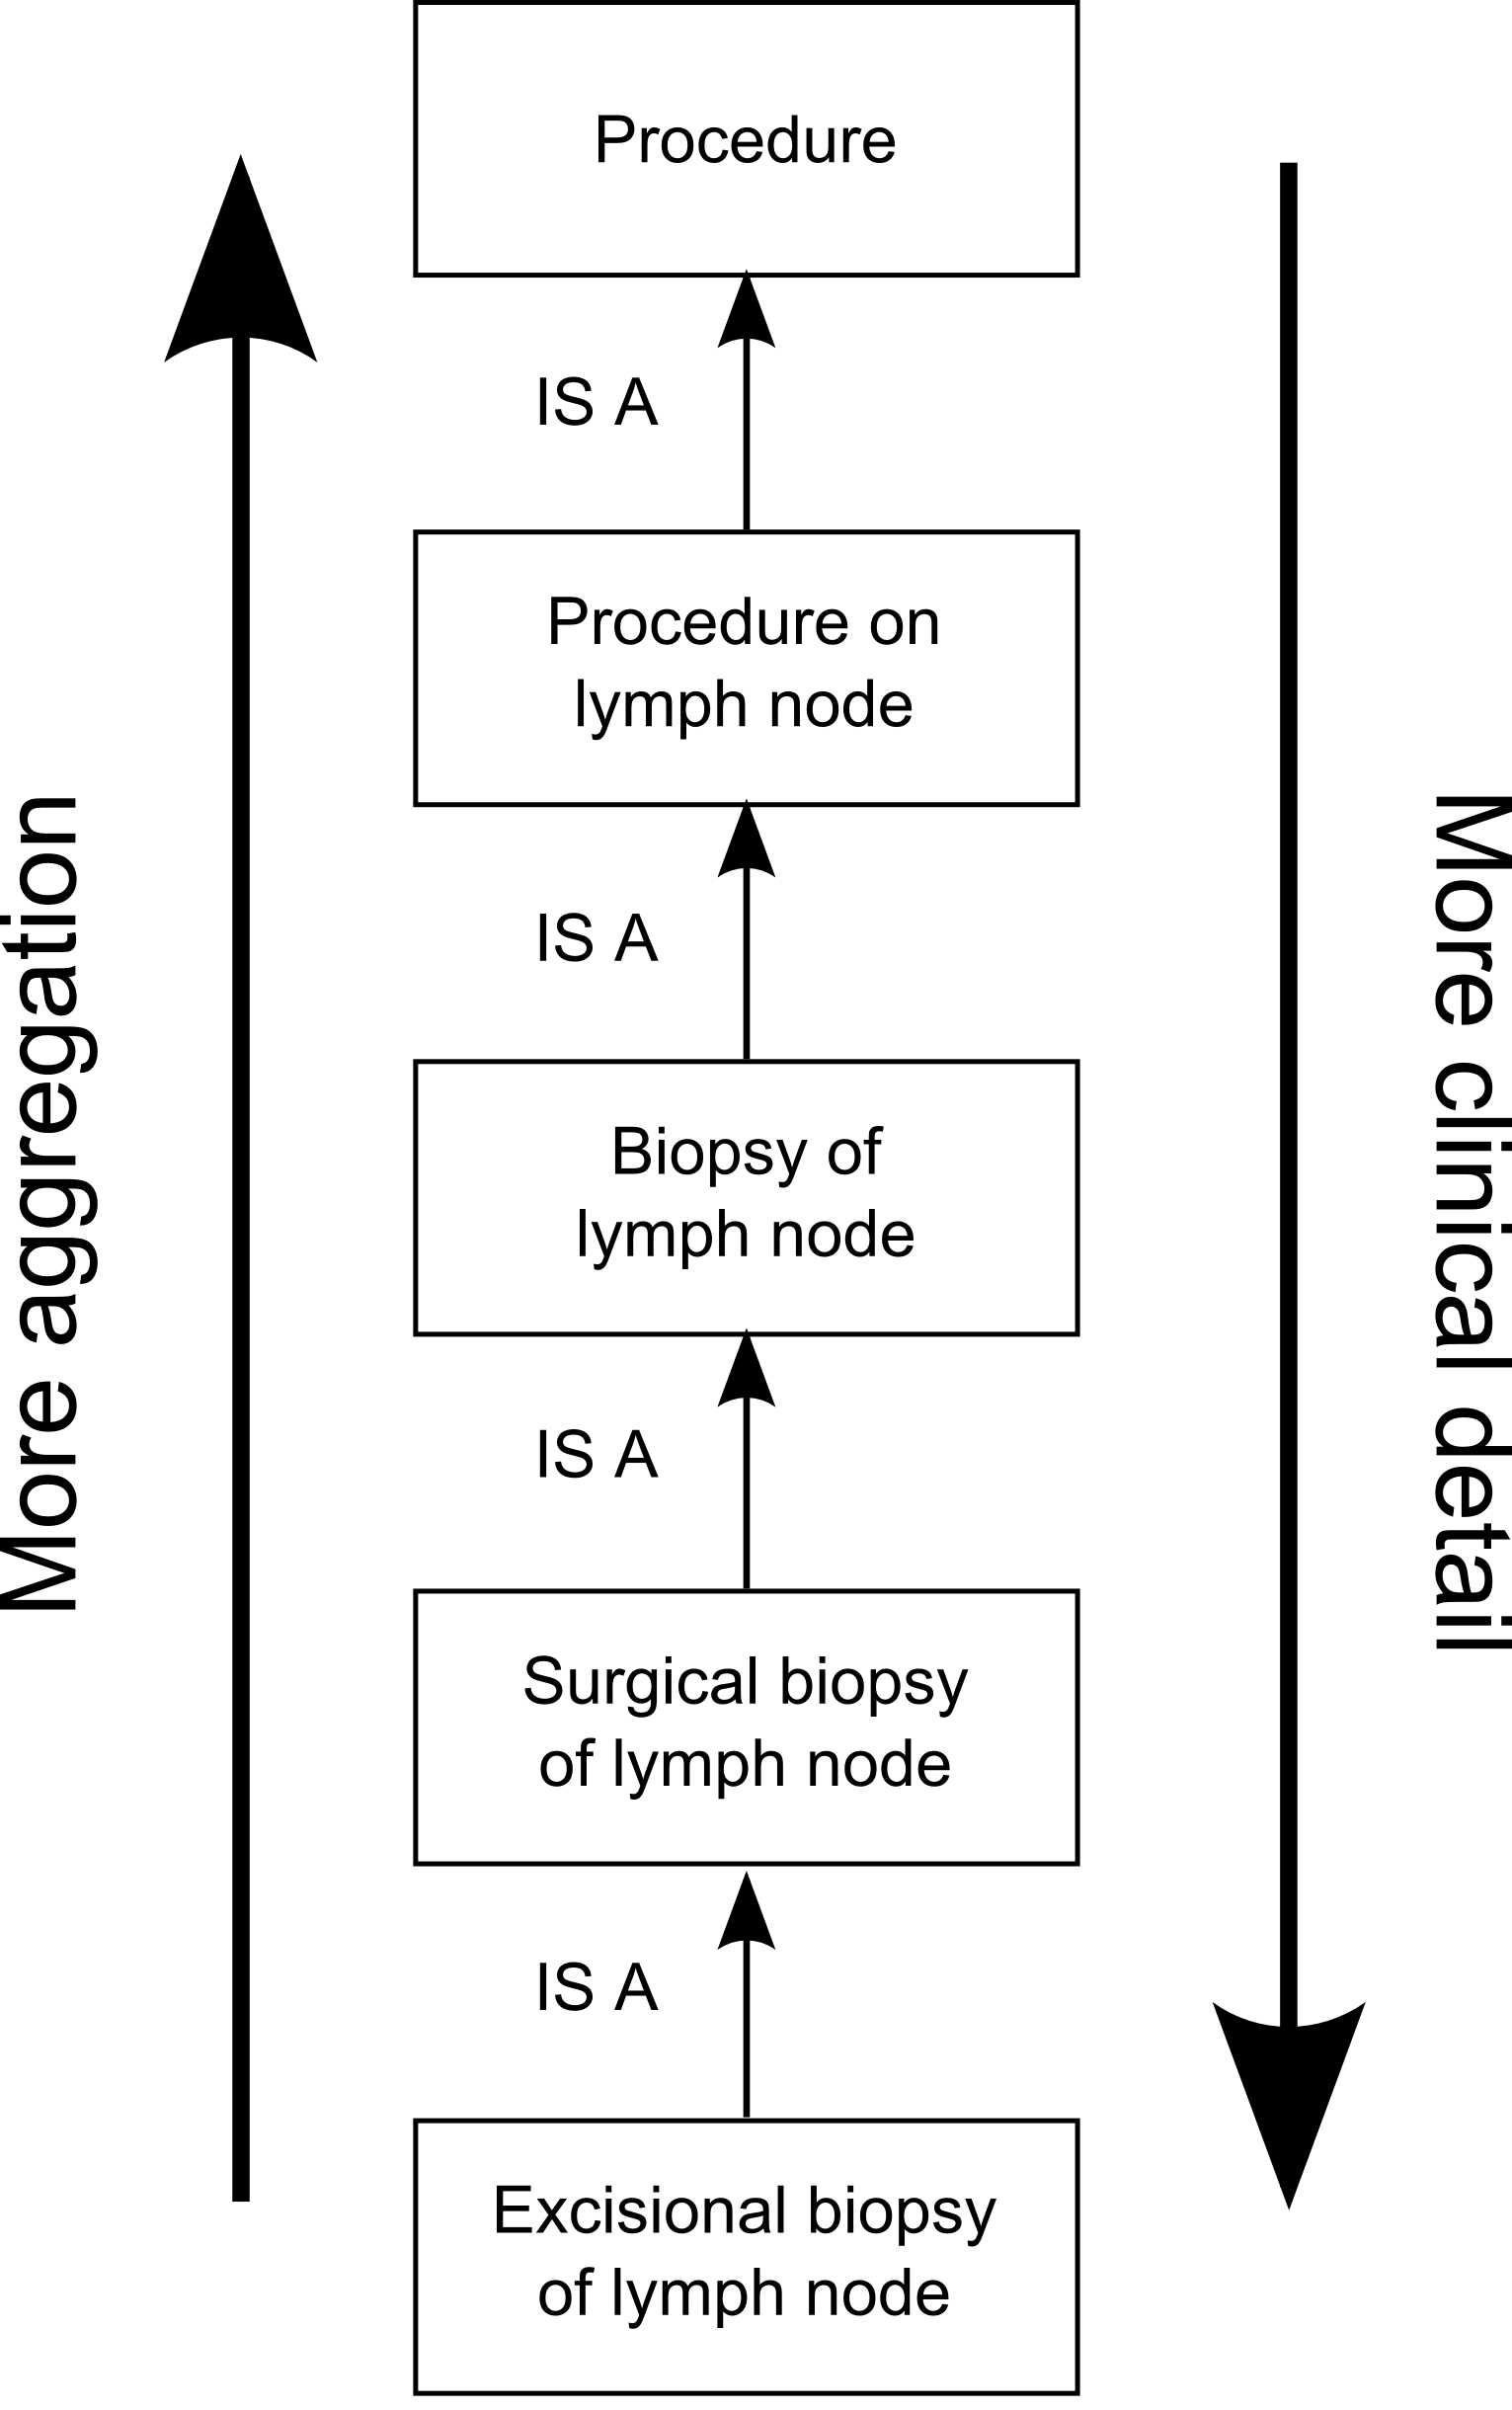
\includegraphics[scale=1]{granularity.png}
    \caption{SNOMED CT - Multiple levels of granularity}\cite[Fig.~1]{snomed_-_user_guide_snomed_2011}
    \label{fig:snomedct_concepts_granularity}
  \end{figure}

  \noindent Concept identifiers in SNOMED CT are meaningless to avoid changes to\
  reflect revised understanding of the nature of a disorder. Meaningless identifiers\
  also enable multiple aspects of meaning to be represented in the same way.\\
  
  \subsection{Descriptions}
  Concept Descriptions are the terms or names assigned to a SNOMED CT concept.\
  A unique DescriptionId  identifies a Description. Multiple Descriptions might be\
  associated with a concept identified by a ConceptId. There are nearly a million\
  English Descriptions in the International Release of SNOMED CT. Each translation\ 
  of SNOMED CT includes an additional set of descriptions, which link terms in another\
  language to the same SNOMED CT concepts.
  
  \noindent\textbf{\emph{Example:}}
  Some of the Descriptions associated with \emph{ConceptId} 22298006:
  \begin{itemize}
    \itemsep0em
    \item{Fully Specified Name: | Myocardial infarction (disorder) | \emph{DescriptionId}\
    751689013}
    \item{Preferred term: Myocardial infarction \emph{DescriptionId} 37436014}
    \item{Synonym: Cardiac infarction \emph{DescriptionId} 37442013}
    \item{Synonym: Heart attack \emph{DescriptionId} 37443015}
    \item{Synonym: Infarction of heart \emph{DescriptionId} 37441018}
  \end{itemize}
  Each of the above Descriptions has a unique \emph{DescriptionId}, and all of these\
  Descriptions are associated with a single Concept (and the single \emph{ConceptId} 22298006).\\

  \subsection{Relationships}
  SNOMED CT Relationships link each concept to other concepts that have a related\
  meaning. These relationships provide formal definitions and other characteristics of\
  the concept. One type of link is the \textbar ~is a \textbar ~relationship which\
  relates a concept to the its more general concepts. For example, the concept\
  ``viral pneumonia'' has an \textbar ~is a \textbar ~relationship to the more\
  general concept ``pneumonia''. These \textbar ~is a \textbar ~relationships\
  define the hierarchy of SNOMED CT concepts. Other types of relationships\
  represent other aspects of the definition of a concept. For example, the concept\
  ``bacterial pneumonia'' has a \textbar ~causative agent \textbar ~relationship to\
  the concept ``bacteria'' and a \textbar ~finding site \textbar ~relationship to the\
  concept ``lung structure''. There are well over a million relationships in SNOMED CT.
  \begin{figure}[!ht]
    \centering
    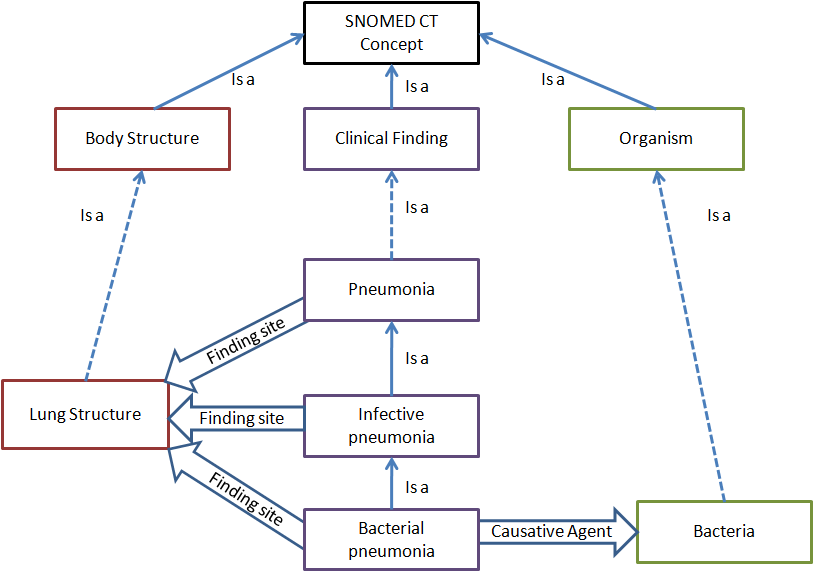
\includegraphics[scale=0.5]{defining_relationship_example1.png}
    \caption{SNOMED CT - Illustration of Defining Relationships}\cite[Fig.~7]{snomed_-_user_guide_snomed_2011}
    \label{fig:snomedct_relationships}
  \end{figure}

\subsection{Implementation}
  SNOMED CT is distributed as a set of tab-delimited text files that can be\
  imported into a relational database. The three tables - the Concepts table,\
  the Descriptions table and the Relationships table are commonly referred to\
  as \emph{Core Components}~\cite{snomed_implementation_guide_snomed_2011}.\
  Supplementary tables called \emph{Reference Sets} specify the common extensible\
  pattern that is used to add additional information related to the core components.

  \subsection{Summary}
  SNOMED CT is a used widely to achieve semantic uniformity\
  and consistency of health terms as well as to achieve interoperability between HL7\
  (Health Level 7) based health frameworks and other healthcare entities as shown\
  by the works in \cite{ryan_towards_2006,arguello_executing_2009,khan_achieving_2012}.\
  Not only does it provide unique semantic identifiers to clinical concepts, SNOMED CT\
  also describes and links different concepts in an ontogolical fashion.\
  While SNOMED CT has emerged internationally as a leading terminology, the work of\
  \cite{he_clinical_2012, khare_exploiting_2012} delineates that the existing SNOMED CT\
  lexicon suffers from a surprisingly huge paucity of synonyms.\
  Efforts are underway to reduce SNOMED CT's structural complexity\
  and provide a metathesaurus of clinical concepts with mappings to different terminologies,\
  thereby improving semantic integrity in practical healthcare scenarios.\
  \cite{lindberg_unified_1993,wei_using_2012}

%----------------------------------------------------------------------------------------
%	RDF
%----------------------------------------------------------------------------------------


 \section[Resource Description Framework (RDF)]{RDF}

\initial{R}\textit{esource Description Framework (RDF)}\
is a World Wide Web Consortium (W3C) standardized data model for representing\
semantic Web resources. It uses graphs to represent information using a triple-based\
 notation comprising a subject, predicate and an object. All these entities can be uniquely identified by Internationalized Resource Identifiers (IRIs).\\

\subsection{How we can use it}

We can use it by evoking already existing tools to transfer relational data that\
already exists into RDF format which will then allow us to easily gain insight between data.\
An example would be the following,

\subsection{Why this model be useful for our application}

\subsection{Comparison with other data models}

%----------------------------------------------------------------------------------------
%	HDD
%----------------------------------------------------------------------------------------

\section[Healthcare Data Dictionary ( HDD) ]{HDD}


%----------------------------------------------------------------------------------------
%	ICD
%----------------------------------------------------------------------------------------

\section[International Classification of Diseases ( ICD ) ]{ICD}

%----------------------------------------------------------------------------------------
%	LOINC
%----------------------------------------------------------------------------------------

\section[Logical Observation Identifier Names and Codes terminology ( LOINC )] {LOINC}

\subsection{How we can use it}

\subsection{How is data stored/API's}

%----------------------------------------------------------------------------------------
%	HL7/FHIR
%----------------------------------------------------------------------------------------

\section[Fast Healthcare Interoperability Resources (HL7/FHIR )]{HL7/FHIR }

%----------------------------------------------------------------------------------------
%	NwHIN
%----------------------------------------------------------------------------------------

\section[Nationwide Health Information Network (NwHIN)]{NwHIN}

%----------------------------------------------------------------------------------------
%	SPARQL
%----------------------------------------------------------------------------------------

\section[SPARQL Protocol and RDF Query Language (SPARQL)]{SPARQL}

\initial{S}\textit{SPARQL Protocol and RDF Query Language (SPARQL}]\
		is a W3C recommend standard for querying RDF data.\
		It allows one to query remote RDF resources, in a manner similar to the querying of databases using SQL.\
		A SPARQL query is a set of graph patterns; any data triple matching these patterns is added to the query results.\\
		
		\subsection{Alternatives}
		SquishQL (http://www.techrepublic.com/article/squishql-the-simplest-rdf-query-language/)//
		
		\subsection{Examples}

%----------------------------------------------------------------------------------------
% 	BIO2RDF
%----------------------------------------------------------------------------------------

\section[Bio2RDF]{Bio2RDF}

%----------------------------------------------------------------------------------------
%	FMQL
%----------------------------------------------------------------------------------------

\section[FileMan Query Language (FMQL)]{FMQL}

\initial{F}\textit{ileMan Query Language (FMQL)}\
is a Query Language that provides access to both FileMan data\
- a vital measurement of a patient - and the schema of that data - the type "Vital Measurement".\
The three things that it addresses are:
\begin{enumerate}
\item
Identity: every entity and entity type in FileMan gets a unique identifier - a URI.
\item
Data Formats: a consistent form of JSON, the web-friendly response format, for every type of data in the system\
 as well as HTML for human readers and RDF for web-data practitioners.
\item
Query Nuance: from the precise - SELECT - to the broader - DESCRIBE - or just COUNT, covers data hierarchies\
 and graphical layouts, paging and filtering.
\end{enumerate}
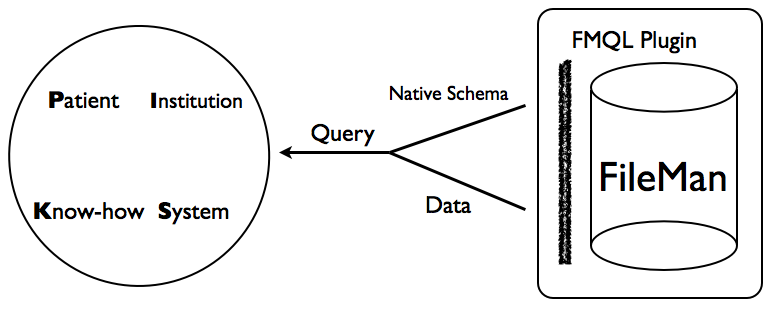
\includegraphics[scale=0.4]{fmqlFromFileMan.png}\\

   %----------------------------------------------------------------------------------------
  %	REFERENCE LIST
  %----------------------------------------------------------------------------------------

  \bibliographystyle{apalike}
  \bibliography{SemanticHealthcare}{}

%----------------------------------------------------------------------------------------

\end{document}
